\documentclass[12pt,letterpaper]{article}
\usepackage[margin=1in]{geometry}
\usepackage[utf8]{inputenc}
\usepackage[T1]{fontenc}
\usepackage{lmodern}
\usepackage{amsmath,amssymb}
\usepackage{setspace}
\usepackage{graphicx}
\usepackage{booktabs}
\usepackage{caption}
\usepackage{float}
\usepackage[round,authoryear]{natbib}
\usepackage[hidelinks]{hyperref}
\usepackage{microtype}

\graphicspath{{../figures/}}
\captionsetup{font={small,stretch=1.0},labelfont=bf,width=0.95\textwidth,skip=4pt}
\setlength{\bibsep}{0pt}
\setlength{\textfloatsep}{8pt}
\setlength{\intextsep}{8pt}
\doublespacing

\title{\large\textbf{Watermarking Large Language Models:\\ A Reproduction of Kirchenbauer et al.\ (2023) and Five Extensions}}
\author{\normalsize Piero Pelosi, Romain Almeida, Elias Roubache\\[0.3em]
\small MFE 230ZB, Generative AI and Causality, UC Berkeley MFE\\
\small Instructor: Prof.\ Ali Kakhbod}
\date{\normalsize October 2026}

\begin{document}
\maketitle
\vspace{-2em}

\begin{abstract}
\singlespacing\noindent
We reproduce the soft green-list watermark of \citet{kirchenbauer2023watermark} with independent code and extend it in five directions. The reproduction is a benchmark: our green lists are identical to the official implementation, the headline detection rate is 98.6\% against the paper's 98.4\%, and 11 of 12 error-rate settings agree within 95\% intervals. We then measure three limits the paper leaves open. The watermark fades on constrained text (code needs 188 tokens to be detected where news needs 24; short factual answers are never detected); one prompt to a free 1.5B-parameter chat model removes it more efficiently than the paper's T5 attack; and a passage pasted into human text is lost in a whole-text count unless a sliding window is used. We also find that the secret key can change how long the model writes. Our main contribution uses the detector as a filter for financial sentiment data. In a synthetic campaign that adds slanted watermarked texts to buckets of human news, dropping the flagged texts restores 95\% of the signal quality for 200-token texts, 40\% at 50 tokens, 7\% at 25, and nothing after a full paraphrase or when the model does not embed the watermark. Recovery equals the detection rate to within 0.03, so every limit measured earlier translates one for one into lost signal quality.
\end{abstract}

\section{Introduction}

Sentiment signals are read from text, and part of that text is now machine-written, some of it to move the signal. Classifiers that guess ``human or AI'' from style have no guaranteed error rate: OpenAI's own classifier caught 26\% of AI text and flagged 9\% of human text before it was withdrawn \citep{openai2023classifier}. \citet{kirchenbauer2023watermark} take the opposite route: the model signs its text while writing, by favouring a secret, context-dependent subset of the vocabulary, and anyone with the key can test for the signature with a $z$-test that needs neither the model nor the prompt. The idea has reached production: Anthropic announced in August 2026 that Claude would watermark its text with a scheme of the same family, with the caveat that it is less reliable on short, factual or code text \citep{anthropic2026watermark}.

This report first reproduces the paper on its own setup and treats the outcome as a benchmark, spending more space on what did not reproduce than on what did. It then presents five extensions. Four measure limits the paper leaves open: constrained text, a modern rewrite attack, a pasted passage, and a side effect of the key. The fifth, our main contribution, asks the question a finance reader cares about: if a manipulated sentiment feed contains watermarked text, how much of the damage does the detector undo? Every number comes from the code and raw outputs in our public repository \citep{repo2026}; square brackets are 95\% intervals (Wilson for rates, percentile bootstrap otherwise).

\section{The method in brief}

Before each token, a hash of the secret key and the previous token seeds a pseudo-random split of the vocabulary into a green list $G$ of size $\gamma|V|$ and a red remainder. The soft watermark adds a bias $\delta$ to the green logits,
\begin{equation}
\hat p_k = \frac{\exp\!\big(l_k + \delta\,\mathbf{1}[k \in G]\big)}{\sum_i \exp\!\big(l_i + \delta\,\mathbf{1}[i \in G]\big)},
\end{equation}
so a green token's odds are multiplied by $e^{\delta}$. Where the model hesitates, green wins; where it is nearly certain, little changes. Detection rebuilds each split from the key and counts green tokens $|s|_G$ among $T$:
\begin{equation}
z = \frac{|s|_G - \gamma T}{\sqrt{T\gamma(1-\gamma)}}, \qquad \text{flag if } z > 4,
\end{equation}
which a human text exceeds with probability $3.2 \times 10^{-5}$. The price is that the signal comes only from tokens where the model had a choice: Theorem 4.2 of the paper bounds the expected green count below by $T\cdot c\cdot S^{\ast}$, with $S^{\ast}$ the average spike entropy of the next-token distribution. That theorem is the thread through our extensions.

\section{Reproduction as a benchmark}

We re-implemented generation, detection, the perplexity oracle and the T5 attack, and ran the paper's setup: C4 news prompts, OPT-1.3B \citep{zhang2022opt} sampling at temperature 0.7, texts of $200 \pm 5$ tokens, OPT-2.7B as quality judge, and T5-Large \citep{raffel2020t5} for the span-replacement attack, whose code was never released. The run took about 20 hours on one laptop. The first check is exact: on 1,000 random contexts our green lists equal the official code's, same ids in the same order, so any remaining gap comes from the experiment and not the implementation. Table~\ref{tab:headline} gives the headline comparison. Across the twelve settings of the paper's Table 8, eleven agree within our intervals (the full table is in the repository); the T5 attack curve has the same shape as the paper's; and after digitising the markers of the paper's Fig.~2 from its arXiv source, our mean $z$ is within 0.78 of the paper's in all 31 matched settings (median gap 0.22).

\begin{table}[htbp]
\centering\singlespacing\small
\caption{Headline setting ($\gamma = 0.5$, $\delta = 2$, $T = 200$): 497 watermarked and 1,000 human texts.}
\label{tab:headline}
\begin{tabular}{lcc}
\toprule
 & Paper & Ours \\
\midrule
Detected at $z = 4$ & 98.4\% & 98.6\% [97.1, 99.3] \\
Human texts flagged & 0 & 0 of 1,000 \\
Mean green tokens of 200 & 159.5 & 158.3 [157.5, 159.2] \\
Theorem 4.2 lower bound & 142.2 & 143.2 \\
Detected at $z = 4$, 4-beam search & 99.6\% & 100\% [97.5, 100] \\
\bottomrule
\end{tabular}
\end{table}

\paragraph{What did not reproduce, and why.} (i) One weak-push setting detects less: multinomial, $\delta = 1$, $\gamma = 0.5$ gives 0.37 [0.31, 0.42] at $z = 5$ against 0.50. With a weak push the signal rests on a few frequent token pairs whose colour the key fixes; our key differs from the paper's (CPU rather than CUDA random generator), and Extension 4 shows how much one key can matter. (ii) The lightest T5 attack removes less in our hands (0.99 against 0.82 still detected at 10\% of words swapped) and heavier ones slightly more; the attack was rebuilt from a prose description, and from 30\% of words on the results agree or come close. (iii) Perplexities sit 0.1 to 1.0 above the paper's. The digitised Fig.~2 shows the offset at $\delta = 0$ too, so it belongs to the oracle run, not the watermark. (iv) OPT-1.3B cannot answer trivia questions, so the Table 10 experiment used Qwen2.5-1.5B-Instruct \citep{qwen2025}; the watermark then costs no measurable accuracy (exact match 0.202 to 0.212), where the paper reports a small loss with far larger models.

\section{Extensions}

The paper's own caveats define the first four extensions; the fifth turns the first three into one number for a sentiment feed. Extension numbers follow our presentation; Appendix~\ref{app:map} maps them to the repository's file names.

\subsection{Extension 1: entropy decides}

The paper evaluates almost only on news. We measured the median number of tokens needed to reach $z = 4$ with OPT-1.3B on news, code (HumanEval, \citealp{chen2021codex}) and short factual answers (TriviaQA, \citealp{joshi2017triviaqa}). News needs 24 tokens [20, 27]; code needs 188 [135, never], and 49\% [42, 57] of functions never reach the threshold within 200 tokens; short answers never do in 99\% of cases, since at $\gamma = 0.5$ a fully green 16-token answer reaches $z = 4$ only exactly (Figure~\ref{fig:ext1}). Two findings qualify this. On code, repeated token pairs break the independence the test assumes; counting each repeated pair once restores calibration and doubles detection at 1\% false positives for Qwen (0.24 to 0.51). And instruction tuning lowers the model's entropy, yet news detection is unchanged: the watermark pushes the instruct model off its confident path, and the cost shows up as quality instead (perplexity 5.7 to 9.5).

\begin{figure}[htbp]
\centering
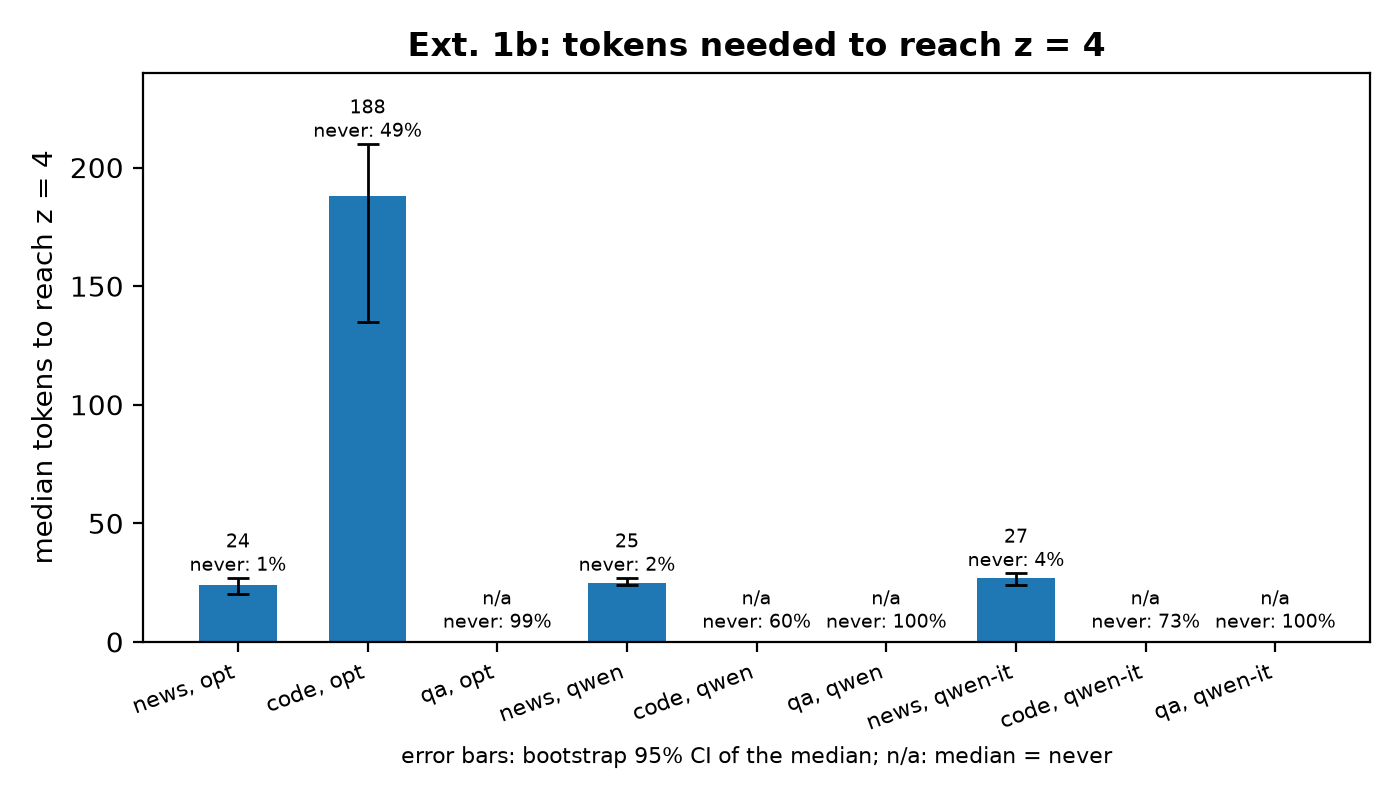
\includegraphics[width=0.7\textwidth]{ext1b_tokens_to_detect.png}
\caption{Extension 1. Median tokens needed to reach $z = 4$ on news, code and short answers, with bootstrap intervals; ``never'' is the share of texts that do not reach the threshold within 200 tokens.}
\label{fig:ext1}
\end{figure}

\subsection{Extension 2: a 2026 attacker}

The paper's attack swaps words with T5, which breaks few of the neighbouring-token pairs the watermark lives in; a rewrite breaks most. We attacked the same 200 watermarked texts with one prompt to Qwen2.5-1.5B-Instruct at three strengths and compared with T5 at matched meaning, measured by the cosine similarity of MiniLM sentence embeddings \citep{reimers2019sbert}; false positives are calibrated on human texts attacked the same way. At the paper's fixed threshold the two attacks are indistinguishable (0.22 against 0.24 still detected). At a calibrated 1\% false-positive rate, which a deployed detector would use, the rewrite is clearly stronger (Table~\ref{tab:ext2}): swapped texts keep $z$-scores just below 4, so a lower threshold catches them, while rewritten texts overlap with human text. Removal still costs meaning, about 15\% of similarity for near-complete removal, but it now takes one call to a free model instead of 60 to 140 T5 calls.

\begin{table}[htbp]
\centering\singlespacing\small
\caption{Extension 2. The same watermarked texts under the paper's attack and a one-prompt rewrite.}
\label{tab:ext2}
\begin{tabular}{lcccc}
\toprule
Attack & Meaning kept & Detected at 1\% FPR & AUC & Model calls \\
\midrule
T5, 30\% of words swapped & 0.856 & 0.81 [0.72, 0.88] & 0.995 & 60 to 140 \\
Qwen, light rewrite & 0.850 & 0.435 [0.37, 0.50] & 0.881 & 1 \\
Qwen, full rewrite & 0.837 & 0.10 [0.07, 0.15] & 0.705 & 1 \\
\bottomrule
\end{tabular}
\end{table}

\subsection{Extension 3: a passage pasted into human text}

We hid one watermarked span of 60, 150 or 300 tokens inside a 600-token human document, with thresholds set for 1\% false positives on 1,000 human-only documents. The surrounding human tokens pull the whole-text count toward chance: a 60-token span is caught 11.5\% [7.8, 16.7] of the time. The sliding-window maximum of the authors' follow-up \citep{kirchenbauer2024reliability} restores the contrast, catching it 86.5\% [81.1, 90.6] of the time; both detectors exceed 99\% from a 150-token span. The open question has an answer in a tool that already exists.

\subsection{Extension 4: the key can change when the model stops}

This was a surprise rather than a planned test. Under our key, after a period the end-of-text token is green while the newline, the usual continuation, is red, so $\delta = 2$ multiplies the chance of stopping by about 2.3: 16\% [14, 18] of watermarked texts end before 50 tokens, against 6\% [4, 7] without the watermark. Under three other keys the multiplier is 0.17, 1.18 and 0.32, and length distributions look normal. The paper's filter keeping only texts of $200 \pm 5$ tokens hides this, and it is our best candidate explanation for the weak-push cell that did not reproduce.

\subsection{Extension 5: the watermark as a filter for sentiment data}

\paragraph{Design.} Media sentiment moves prices \citep{tetlock2007}, and a signal built from many texts can be pushed by adding machine-written ones. If the added texts carry the watermark, a data vendor can drop every text the detector flags. We measure how much of the damage this undoes, between two bounds: no filter (worst) and a perfect filter that removes every AI text (best). Sentiment is scored once per text with FinBERT \citep{araci2019finbert}, $S = P(\text{positive}) - P(\text{negative})$, a classifier separate from the generator. A bucket stands for one day of text on one subject: 50 human news texts drawn from the paper's 1,000 human baselines, whose mean $S$ is the truth. In 50 of 100 buckets an attacker adds AI texts until they make up a share $c \in \{0.1, 0.3\}$, pushing up in half (the top third of the AI pool by $S$) and down in the other half. Errors over buckets are the RMSE and the Spearman correlation against the truth, and
\begin{equation}
\text{recovery} = 1 - \frac{\text{RMSE}_{\text{filtered}} - \text{RMSE}_{\text{perfect}}}{\text{RMSE}_{\text{none}} - \text{RMSE}_{\text{perfect}}} .
\end{equation}
The draw is repeated 500 times. No new text was generated: the AI texts are the headline watermarked texts cut to 25, 50, 100 and 200 tokens, with $z$ recomputed from the stored green ranks, the Extension 2 paraphrases, the unwatermarked generations, and the Extension 3 documents. If escaping the filter is unrelated to sentiment, recovery is a function of the detection rate $p$ alone; we test this (H5) against a sentiment-blind filter that removes exactly as many AI texts with shuffled identities, inside the same draws. The interesting failure would be if constrained, low-entropy text both escaped the detector and read as flat.

\begin{figure}[htbp]
\centering
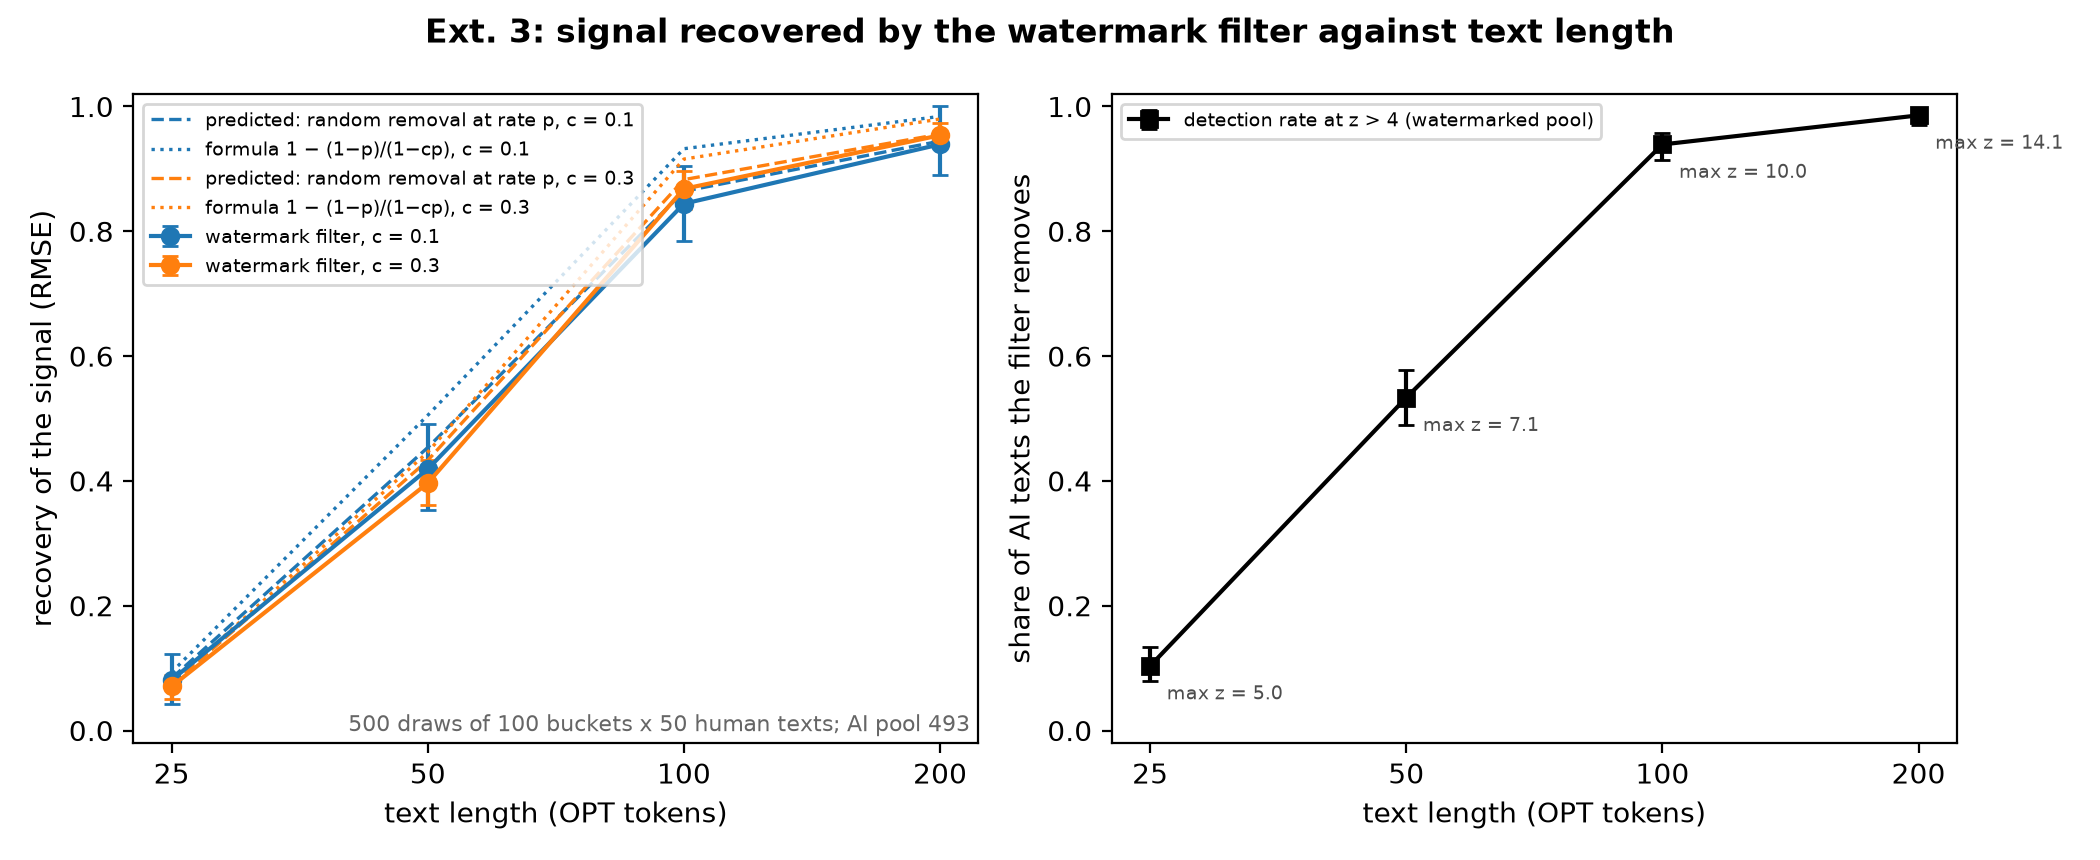
\includegraphics[width=0.62\textwidth]{ext3_recovery_vs_length.png}
\caption{Extension 5. Recovery of the sentiment signal against text length for watermarked texts at the fixed threshold $z > 4$, with the prediction from the detection rate alone. Percentile intervals over 500 re-draws of 100 buckets.}
\label{fig:ext5}
\end{figure}

\begin{table}[htbp]
\centering\singlespacing\footnotesize
\caption{Extension 5 at contamination share $c = 0.3$. ``Predicted'' removes the same number of AI texts with shuffled identities (H5); every interval of the last column covers zero.}
\label{tab:ext5}
\setlength{\tabcolsep}{4pt}
\begin{tabular}{llccccc}
\toprule
AI texts & Tokens & $p$ & RMSE none / filter & Recovery [95\%] & Predicted & Actual $-$ pred. \\
\midrule
watermarked & 25 & 0.103 & 0.076 / 0.070 & 0.071 [0.051, 0.089] & 0.071 & $-0.001$ \\
watermarked & 50 & 0.533 & 0.088 / 0.053 & 0.397 [0.361, 0.434] & 0.417 & $-0.021$ \\
watermarked & 100 & 0.939 & 0.089 / 0.012 & 0.868 [0.836, 0.896] & 0.895 & $-0.027$ \\
watermarked & 200 & 0.986 & 0.083 / 0.004 & 0.954 [0.938, 0.973] & 0.976 & $-0.022$ \\
light paraphrase & 151 & 0.220 & 0.108 / 0.092 & 0.149 [0.130, 0.167] & 0.169 & $-0.020$ \\
full paraphrase & 178 & 0.015 & 0.117 / 0.116 & 0.006 [0.004, 0.008] & 0.011 & $-0.005$ \\
no watermark & 200 & 0.002 & 0.082 / 0.082 & 0.000 [0.000, 0.000] & 0.000 & 0.000 \\
\bottomrule
\end{tabular}
\end{table}

\paragraph{What worked.} Contamination harms the signal: at $c = 0.3$ the rank correlation with the truth falls from 1 to 0.45. On long, unattacked text the filter undoes 0.95 [0.94, 0.97] of the damage and brings the correlation back to 0.996. Recovery falls with length in step with detection, 0.07, 0.40, 0.87, 0.95 at 25, 50, 100, 200 tokens (Figure~\ref{fig:ext5}, Table~\ref{tab:ext5}), and collapses after a rewrite: 0.15 after a light edit, under 0.01 after a full paraphrase. The detector removes none of the 5,000 human texts in any draw. H5 is not rejected: actual minus predicted recovery lies between $-0.03$ and $0.00$ in all 16 cells and every interval covers zero. So recovery is the detection rate to within 0.03, and Extensions 1 to 3, which measured lost detection, read directly as lost signal quality. Two results matter for a vendor. A threshold calibrated to 1\% false positives on human text of the same length lifts recovery at 25 tokens from 0.07 to 0.63 and at 50 tokens from 0.40 to 0.90, for about 20 human texts lost in 5,000. And on 60-token passages pasted into human documents, the sliding-window detector recovers 0.66 [0.57, 0.73] where the whole-text test recovers nothing.

\paragraph{What did not work, and why.} The honest limit is unwatermarked AI text: the filter removes none of it and recovery is exactly zero, so the filter is worth what the provider's cooperation is worth. At 25 tokens the fixed threshold binds, since the largest attainable $z$ is $\sqrt{T} = 5$; the calibrated threshold fixes this, but its realised false-positive rate is 0.3 to 0.4\% rather than 1\% because $z$ is discrete at short lengths. The point estimates of actual minus predicted recovery are all slightly negative: the texts that escape at 50 and 100 tokens are, if anything, a little more extreme than their pool, the opposite of the flattening we looked for, and too small to matter. The slanted pools are small (164 texts per direction, 66 for the paraphrases) and reused across buckets, which we accepted rather than generating new text; this is why the simpler prediction that removes texts independently at rate $p$ is too pessimistic in the pasted-passage scenario, where a fixed handful of escapers makes the per-bucket count less variable than a binomial. The shuffled prediction removes most of that gap. FinBERT labels 71 to 74\% of general news neutral, leaving the slant less room than a domain-matched classifier would. Finally, the campaign is synthetic: we select slanted texts rather than prompting for slant, and a prompted campaign could produce lower-entropy, harder-to-detect text, the one mechanism this design cannot reach.

\section{Discussion and conclusion}

The reproduction holds: with independent code the paper's headline, error-rate table and attack curve come back within sampling error, and the gaps have identifiable causes in the key, the oracle run, or an attack rebuilt from prose. The extensions sharpen the paper's own caveat: the watermark is a function of entropy, so it fades where a reader might want it most; a free model removes it in one call; a pasted passage needs a window test; and the key can change the length of what the model writes. Extension 5 turns these into one number: the share of a manipulated signal that a watermark filter gives back equals the detection rate, 95\% for long, unattacked text from a cooperating provider, and small or zero for short snippets, rewritten text, or a model that does not watermark. A vendor relying on this filter should calibrate its threshold on human text of the lengths it actually sees, use a window test for mixed documents, and treat the filter as a complement to provenance from the source, not a replacement.

\smallskip
\noindent{\small\textbf{Use of AI tools.} Claude Code wrote the code and ran the experiments under our specifications; we chose the paper, the extensions and the checks, reviewed every result, and wrote this report.}

\singlespacing
{\small
\bibliographystyle{plainnat}
\bibliography{refs}}

\appendix
\section{Deviations, compute and naming}
\label{app:map}

\small
\textbf{Deviations.} Green lists use a CPU random generator, as the official code does on CPU, so the concrete lists differ from the paper's CUDA runs while the scheme and statistics are identical. Each configuration is filtered on its own length (195 to 205 tokens). The T5 attack follows the paper's description (T5-Large in bfloat16, $\pm 60$-token windows, 50-beam search with 20 candidates, one word per replacement). Perplexity is computed on token ids. The 8-beam rows beyond $\delta = 2$ use 100 texts rather than about 500. The 1\% false-positive thresholds of Extension 2 come from 100 to 200 attacked human texts and are noisy; the AUC supports the same comparison. The null distribution of $z$ is key-specific (mean $z$ of unwatermarked text from $-0.52$ to $+0.71$ across six keys), so deployed thresholds should be calibrated empirically, as every 1\%-FPR number here is.

\textbf{Compute.} About 20 hours on one Apple M5 Pro laptop (24~GB, fp16), dominated by the T5 attacks (9~h) and 8-beam search (6~h). Extension 5 needed no generation: FinBERT scoring took 33 seconds and each simulation block under 40 seconds.

\textbf{Naming.} In the repository, Extension 1 is labelled 1a to 1c, Extension 2 is 2a, Extension 3 is 2b, Extension 4 is the key and length check, and Extension 5 lives under \texttt{ext3\_filter} (\texttt{SPEC\_ext3\_filter.md}, \texttt{PLAN\_ext3.md}, \texttt{HANDOFF\_ext3.md}). The notebook rebuilds every table and figure from the raw outputs in about a minute; \texttt{python run.py list} prints the pipeline.

\end{document}
